\documentclass[border=1pt]{standalone}


\usepackage{tikz}
\usetikzlibrary{arrows, decorations.markings}
\usetikzlibrary{shapes,snakes}
\usetikzlibrary{decorations.pathmorphing}	% For Feynman Diagrams
\usetikzlibrary{decorations.markings}
\usetikzlibrary{decorations.text}

%Some nicer color definitions
\definecolor{crimsonred}{RGB}{153,0,0}		% Neurtal red, good for dark or light bg
\definecolor{darkcharcoal}{RGB}{25,25,25}		% Darker gray
\definecolor{charcoal}{RGB}{51,51,51}		% Darker gray
\definecolor{ash}{RGB}{100,100,100}			% medium gray
\definecolor{paleblue}{RGB}{0,102,102}		% More of an `ocean' color
\definecolor{turtlegreen}{RGB}{51,153,0}	% A more neutral green
\definecolor{paleale}{RGB}{204,204,102}		% Only for dark BG
\definecolor{lager}{RGB}{140,110,10}		% Use instead of pale ale for white BG
\definecolor{regal}{RGB}{90,0,120}			% A more neutral purple
\definecolor{jeans}{RGB}{20,30,150}			% A more neutral blue
\definecolor{Alert}{RGB}{51,153,0}	

%Definitions for drawing feynman diagrams
\tikzset{
    vector/.style={decorate, decoration={snake}, draw=Alert},
	provector/.style={decorate, decoration={snake,amplitude=2.5pt}, draw},
	antivector/.style={decorate, decoration={snake,amplitude=-2.5pt}, draw},
    fermion/.style={draw=jeans, postaction={decorate},
        decoration={markings,mark=at position .55 with {\arrow[draw=jeans]{>}}}},
    fermionbar/.style={draw=jeans, postaction={decorate},
        decoration={markings,mark=at position .55 with {\arrow[draw=jeans]{<}}}},
    fermionnoarrow/.style={draw=black},
    gluon/.style={decorate, draw=lager,
        decoration={coil,amplitude=4pt, segment length=5pt}},
    scalar/.style={dashed,draw=black, postaction={decorate},
        decoration={markings,mark=at position .55 with {\arrow[draw=black]{>}}}},
    scalarbar/.style={dashed,draw=black, postaction={decorate},
        decoration={markings,mark=at position .55 with {\arrow[draw=black]{<}}}},
    scalarnoarrow/.style={dashed,draw=black},
    electron/.style={draw=jeans, postaction={decorate},
        decoration={markings,mark=at position .55 with {\arrow[draw=black]{>}}}},
     bigvector/.style={decorate, decoration={snake,amplitude=4pt}, draw},
     line/.style={decorate, draw=black},
}

\tikzset{
    partial ellipse/.style args={#1:#2:#3}{
        insert path={+ (#1:#3) arc (#1:#2:#3)}
    }
}

\begin{document}

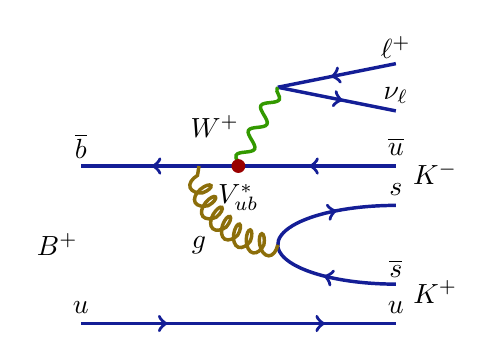
\begin{tikzpicture}[line width=1.25 pt, scale=1]
\draw[fermion]  (1,0) -- (-1,0) ;
\draw[fermion]  (3,0) -- (1,0) ;

\draw[fermion]  (-1,-2) -- (1,-2) ;
\draw[fermion]  (1,-2) -- (3,-2) ;

\draw[fermion]  (1.5+1.5, 1+0.3) -- (1.5, 1);
\draw[fermion]  (1.5, 1) -- (1.5+1.5, 1-0.3) ;
\draw[vector]  (1,0) -- (1.5, 1) ;

\draw[fermion] (3,-1) [partial ellipse=181:90:1.5cm and 0.5cm];
\draw[fermion] (3,-1) [partial ellipse=270:179:1.5cm and 0.5cm];

\draw[gluon] (1.5,0) [partial ellipse=270:180:1cm and 1cm];
\node at (0.5, -1) {$g$};

\node at (-1, 0.25) {$\overline b$};
\node at (3, 0.25) {$\overline u$};

\node at (-1, -1.8) {$u$};
\node at (3, -1.8) {$u$};
\node at (3, -2) {};

\node at (3, -1.3) {$\overline s$};
\node at (3, -0.3) {$s$};

\node at (3, 1.5) {$\ell^{+}$};
\node at (3, 0.9) {$\nu_\ell$};

\node at (-1.3, -1) {$B^{+}$};
\node at (3.5,-0.1) {$K^{-}$};
\node at (3.5,-1.6) {$K^{+}$};

\draw (1,0) node[circle,inner sep=0pt,minimum size=5pt,fill=crimsonred]{};
\node at (1, -0.4) {$V_{ub}^{*}$};
\node at (0.7, 0.5) {$W^{+}$};

\end{tikzpicture} 



\end{document}